%====================================================================
\subsection{Dimension reduction}
%====================================================================
\frame{\frametitle{Dimension reduction (PCA)} \pause

  \paragraph{Dimension reduction.} 
  \begin{itemize}
    \setlength{\itemsep}{0.5\baselineskip}
  \item Metagenomic, metabarcoding, environmental genomics: $p = 10^2, 10^3$ species.
  \item (Probabilistic) PCA \refer{Tib99}: the latent dimension of the data is actually $q \ll p$.
  \end{itemize}
  
  \pause \bigskip \bigskip 
  \paragraph{PLN-PCA model = reduced latent dimension.}  \refer{CMR18a}
  \begin{itemize}
    \setlength{\itemsep}{0.5\baselineskip}
    \item Do not need a latent vector $Z_i$ with $p$ free coordinates in each site. 
    \item \pause A latent vector $W_i$ with $q \ll p$ free coordinates suffices:
    $$
    W_i = [W_{i1} \; \dots \; W_{iq}] \sim \Ncal(0, I_q).
    $$ 
    \item \pause $Z_i$ can then be reconstructed from $W_i$ as $Z_i = B W_i$, where $B: p \times q$.
  \end{itemize}

  \pause \bigskip
  \ra The covariance matrix $\Sigma$ has rank $q \ll p$: 'low-rank' approximation.
  
  \pause \bigskip \bigskip 
  \paragraph{Model selection.} The latent dimension $q$ can be selected using standard criteria (BIC, ICL, ...).

}

%====================================================================
\frame{\frametitle{Oak powdery mildew dataset (1/2)}

  \bigskip 
  \paragraph{Metabarcoding data.} \refer{JFS16} 
  \begin{itemize}
    \setlength{\itemsep}{1\baselineskip}
    \item $p = 114$ OTUs (bacteria and fungi) \\ 
      \ra different extraction protocol for each group.
    \item $n = 116$ leaves = samples \\
      \ra collected from 3 different trees, at different positions in the tree.
    \item $Y_{ij} =$ read count for species $j$ in sample $i$.
  \end{itemize}
  
  \pause \bigskip \bigskip 
  \paragraph{Questions.}
  \begin{itemize}
    \setlength{\itemsep}{0.5\baselineskip}
    \item Effect of the covariates (tree, position) on the abundance of the species.
    \item Visualization.
    \item Account for the heterogeneity of the sampling protocol.
  \end{itemize}

  \pause \bigskip \bigskip 
  \paragraph{Use of the offset.}
  $$
  o_{ij} = \log(\text{total sequencing depth of sample $i$ for the group of species $j$}).
  $$
}

%====================================================================
\frame{\frametitle{Oak powdery mildew dataset (2/2)}

  $$
  \begin{tabular}{c}
    \includegraphics[height=.38\textheight]{\fignet/CMR18-AnnApplStat-Fig4a} \\
    \pause ~ % \\
    \includegraphics[height=.38\textheight]{\fignet/CMR18-AnnApplStat-Fig5a} 
  \end{tabular}
  $$
  \pause
  \ra Other main effects = distance to the ground, then orientation. 
}

%====================================================================
\frame{\frametitle{Microbiote of young pigs}

  \paragraph{Data.} \refer{MBE15}
  \begin{itemize}
    \item $n = 155$ piglets, 
    \item $p = 500$ OTUs ($= 90\%$ of the total abundance of the original 4031 OTU)
  \end{itemize}
  
  \pause \bigskip \bigskip 
  \paragraph{Question.} 
  Effect of weaning

  \pause \bigskip \bigskip 
  \paragraph{PLN-PCA.} No covariate:
  $$
  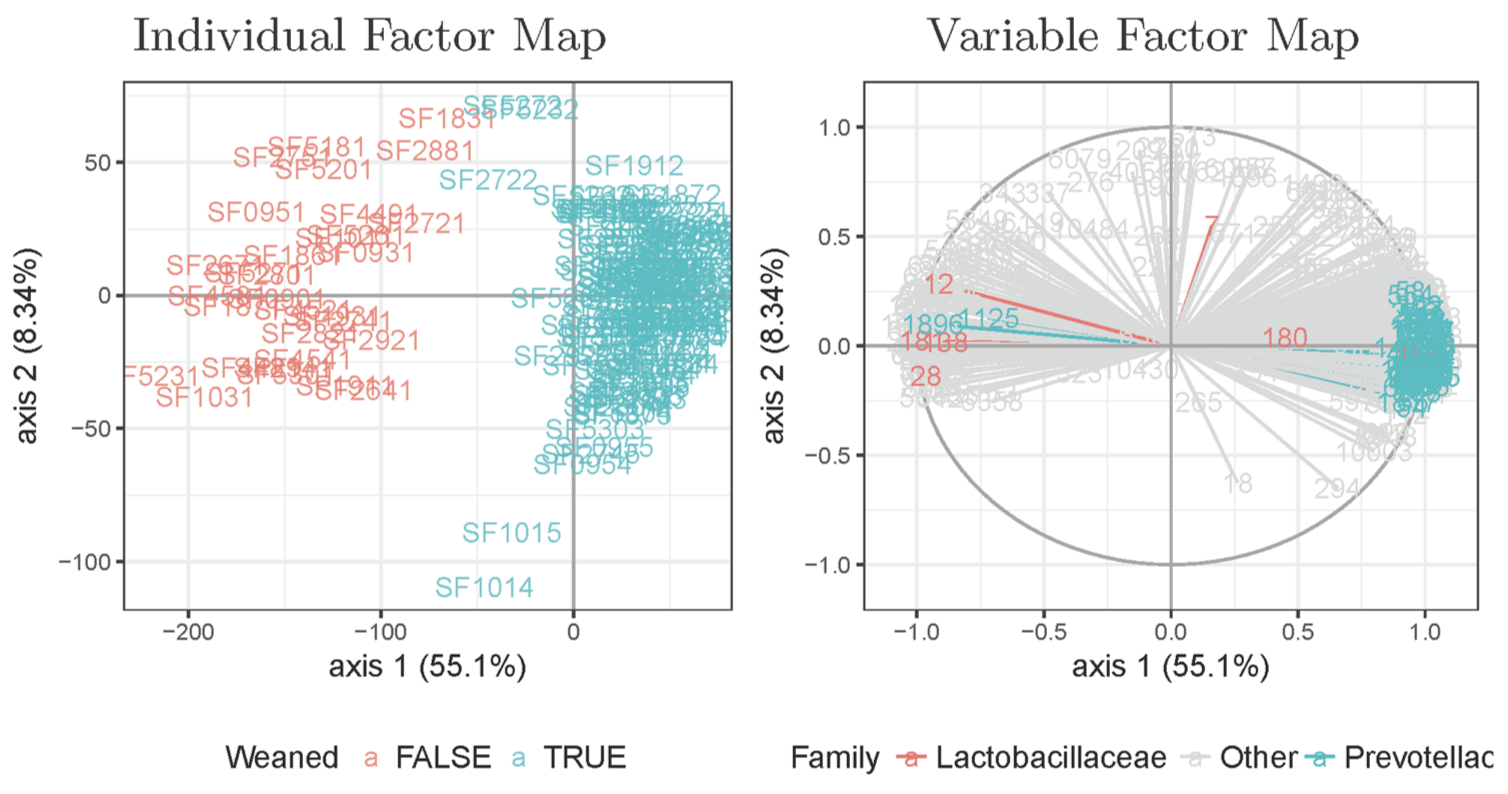
\includegraphics[height=.45\textheight]{\figeco/CMR18-AnnApplStat-Fig3}
  $$  

}

